% v2-acmsmall-sample.tex, dated March 6 2012
% This is a sample file for ACM small trim journals
%
% Compilation using 'acmsmall.cls' - version 1.3 (March 2012), Aptara Inc.
% (c) 2010 Association for Computing Machinery (ACM)
%
% Questions/Suggestions/Feedback should be addressed to => "acmtexsupport@aptaracorp.com".
% Users can also go through the FAQs available on the journal's submission webpage.
%
% Steps to compile: latex, bibtex, latex latex
%
% For tracking purposes => this is v1.3 - March 2012

%\documentclass[prodmode,acmtecs]{acmsmall} % Aptara syntax
\documentclass[final,10pt]{article}
% Package to generate and customize Algorithm as per ACM style
%\usepackage[ruled]{algorithm2e}
%\renewcommand{\algorithmcfname}{ALGORITHM}
% \SetAlFnt{\small}
% \SetAlCapFnt{\small}
% \SetAlCapNameFnt{\small}
% \SetAlCapHSkip{0pt}
% \IncMargin{-\parindent}
\usepackage{graphicx}
\usepackage{url}
\usepackage{hyperref}
\usepackage{eurosym}
\usepackage{colortbl}
\usepackage{dcolumn,longtable,hhline,colortbl}
\usepackage[table]{xcolor}
\usepackage{verbatim}
% % Metadata Information
% \acmVolume{-}
% \acmNumber{-}
% \acmArticle{-}
% \acmYear{2016}
% \acmMonth{1}

% Document starts
\begin{document}

% Page heads
%\markboth{G. Zhou et al.}{A Multifrequency MAC Specially Designed for WSN Applications}

% Title portion
\title{Com es decideix a \texttt{decidim.barcelona}?}
\author{Vicen\c{c} G\'omez}
%\affil{Universitat Pompeu Fabra}}
% NOTE! Affiliations placed here should be for the institution where the
%       BULK of the research was done. If the author has gone to a new
%       institution, before publication, the (above) affiliation should NOT be changed.
%       The authors 'current' address may be given in the "Author's addresses:" block (below).
%       So for example, Mr. Abdelzaher, the bulk of the research was done at UIUC, and he is
%       currently affiliated with NASA.

%\begin{abstract}
%\end{abstract}
\date{Premis a projectes innovadors per a la Qualitat Democr\`atica 2017
%(proposta de projecte)
} 
\maketitle
\section{Resum del projecte (m\`axim 300 paraules)}
%<<<<<<< HEAD
%<<<<<<< HEAD
%Decidim Barcelona \'es la plataforma que l'Ajuntament de Barcelona va posar en marxa al Febrer del 2016. Una primera etapa de participaci\'o on-line ha donat lloc a un total de 10,860 propostes que han servit per elaborar 1,467 actuacions incloses en el nou pla d'actuaci\'o municipal. En aquest projecte es proposa el desenvolupament i l'aplicaci\'o de m\`etodes computacionals i estad\'istics per extreure coneixement del volum de dades recol$\cdot$lectades a la plataforma durant el primer per\'iode de funcionament. L'an\`alisi t\'e dos objectius principals:
%=======
%% Decidim Barcelona \'es la plataforma que l'Ajuntament de Barcelona va posar en marxa al Febrer del 2016. Una primera etapa de participaci\'o on-line ha donat lloc a un total de 10,860 propostes que han servit per elaborar 1,467 actuacions incloses en el nou pla d'actuaci\'o municipal. En aquest projecte es proposa el desenvolupament i l'aplicaci\'o de m\`etodes computacionals i estad\'istics per extreure coneixement del volum de dades recol$\cdot$lectades a la plataforma durant el primer per\'iode de funcionament. L'an\`alisi t\'e dos objectius principals:
%
%Decidim Barcelona \'es la plataforma de participaci\'o que l'Ajuntament de Barcelona va posar en marxa al Febrer del 2016. El primer proc\'es ha estat l'elaboraci\'o del Pla d'Actuaci\'o Municipal i ha donat lloc a un total de 10,860 propostes que han servit per elaborar 1,467 actuacions\footnote{\url{}https://decidim.barcelona/processes/pam}. En aquest projecte es proposa el desenvolupament i l'aplicaci\'o de m\`etodes computacionals i estad\'istics per extreure coneixement del volum de dades recol$\cdot$lectades a la plataforma durant el primer per\'iode de funcionament. L'an\`alisi t\'e dos objectius principals:
% 
%>>>>>>> e6a7409b6d28f94d6527dde0432aac60ba920d0b
%=======
Decidim Barcelona \'es la plataforma de participaci\'o ciutadana que l'Ajuntament de Barcelona va posar en marxa al Febrer del 2016. El primer proc\'es ha estat l'elaboraci\'o del Pla d'Actuaci\'o Municipal\footnote{\url{https://decidim.barcelona/processes/pam}} i ha donat lloc a un total de 10,860 propostes que han servit per elaborar 1,467 actuacions incloses en el nou pla d'actuaci\'o municipal. En aquest projecte es proposa el desenvolupament i l'aplicaci\'o de m\`etodes computacionals i estad\'istics per extreure coneixement del volum de dades recol$\cdot$lectades a la plataforma durant el primer per\'iode. L'an\`alisi t\'e dos objectius principals:
%>>>>>>> 4b39f5cae90350b18cc52cc4a9e45b3899b19495
\begin{itemize}
\item
D'una banda, identificar i corregir el biaix selectiu intr\'insic a la plataforma degut a l'escletxa digital. 
Segons un informe recent, un de cada quatre ciutadans \'es usuari b\`asic o espor\`adic d'Internet. 
Aix\'o implica que les dades de participaci\'o no s\'on una mostra fiable.
\item
El segon objectiu consisteix en caracteritzar mitjan\c{c}ant t\`ecniques d'infer\`encia Bayesiana
el proc\'es de decisi\'o que ha donat lloc a l'acceptaci\'o o rebuig de les propostes de la plataforma.
L'an\`alisi consistir\`a en aprendre un model estad\'istic a partir de les dades associades a cada proposta on es tinguin en compte par\`ametres ex\`ogens a la plataforma.
\end{itemize}
Aquests resultats serviran per millorar l'enteniment sobre el comportament col$\cdot$lectiu en la plataforma, identificar possibles intervencions futures per tal d'incloure sectors de la poblaci\'o infra-representats i en general millorar el rendiment de la plataforma en el futur.

\section{Marc conceptual de la proposta}
Un dels reptes actuals m\'es importants \'es com donar sentit als grans volums de dades que la nostra societat genera cont\'inuament.
Les xarxes socials, la medicina personalitzada o els sistemes de recomanaci\'o,% o les ciutats intel$\cdot$ligents, 
que ja formen part de la nostra vida quotidiana, en s\'on clars exemples. 

Aquest projecte considera aquest repte en el marc de la democr\`acia directa.
En Febrer del 2016, l'Ajuntament de Barcelona va encetar la plataforma \texttt{decidim.barcelona}.
Aquesta plataforma ha donat cabuda als processos de participaci\'o ciutadana elaborats durant el mandat.
\'Es una plataforma construida amb eines lliures, similar a la plataforma \texttt{decide.madrid}, desenvolupada
per l'Ajuntament de Madrid.

El proc\'es participatiu iniciat pel Ajuntamentt %govern de Barcelona en Com\'u
ha tingut com a objectiu 
fer els ciutadans part\'iceps d'un proc\'es on tingu\'essin la possibilitat d'evaluar i discutir les propostes realitzades pel govern, aix\'i com oferir la possibilitat de crear de noves.
Durant l'elaboraci\'o del pla estrat\`egic, la plataforma~\texttt{decidim.barcelona} ha perm\'es registrar, visualitzar i interaccionar amb les propostes institucionals i ciutadanes.

El proc\'es de participaci\'o s'ha desenvolupat tant de manera presencial mitjan\c{c}ant reunions com de manera online en la plataforma digital. 
Les reunions s'han caracteritzat per l'esfor\c{c} de fer arribar la participaci\'o a tots els diferents \`ambits territorials de la ciutat, donant lloc a $410$ reunions presencials entre Gener i Abril de 2016, on van assistir un total de $11,577$ persones i $2,099$ organitzacions.
Es calcula que la participaci\'o presencial durant la primera etapa ha estat aproximadament d'un $43\%$.
La resta de participaci\'o, el $57\%$ aproximadament s'ha donat a trav\'es de la plataforma online \texttt{decidim.barcelona}. 

Els resultats d'una primera etapa de participaci\'o s\'on $10,859$ propostes que han rebut $165,087$ suports i $18,191$ comentaris.
%El $42\%$ d'aquestes propostes s\'on a escala de ciutat i el $58\%$ a escala de districte.
%per tal de desenvolupar noves eines.

De moment, han donat lloc a la definici\'o de possibles actuacions, incloses en el Pla d'Actuaci\'o Municipal.
El proc\'es de definici\'o de les actuacions ha estat portat a terme per l'equip de govern i ha incl\`os la revisi\'o, agrupaci\'o i reelaboraci\'o de les propostes provinents de la ciutadania (organitzada i no organitzada) juntament amb les cites presencials i de l'Ajuntament.
Les actuacions s'han definit tenint en compte els continguts de les propostes, el suport que han rebut, els comentaris realitzats i les cites presencials associades.
Aquestes actuacions tenen relacionades una o m\'es propostes i cada proposta acceptada est\`a incloses en una (o m\'es) actuaciones del pla.

Com a exemple, la proposta acceptada amb m\'es suports ($1,720$) ha estat el \emph{Cubriment de la Ronda de Dalt al seu pas per la Vall d'Hebr\'on}. Aquesta proposta ha quedat inclosa en diferents actuacions: (1) \emph{Processos participatius per a la transformaci\'o de l’avinguda Meridiana i la ronda de Dalt}, (2) \emph{Ronda de Dalt als barris d'Horta-Guinard\'o} i (3) \emph{Transformar la ronda de Dalt}. Al mateix temps, l'actuaci\'o (1) inclou quatre propostes m\'es relacionades (possiblement similars) a la proposta del cobriment de la ronda de dals, com per exemple,
\emph{Instal$\cdot$laci\'o fixa d'estaci\'o control contaminaci\'o ambiental a la Ronda de Dalt/Av. Meridiana}.
Per les propostes rebutjades es dona una breu explicaci\'o on s'explica possibles motius pels quals la proposta no s'ha acceptat.

Aquestes dades representen una oportunitat \'unica per analitzar les demandes i interessos col$\cdot$lectius a Barcelona.
La motivaci\'o d'aquesta proposta \'es precissament desenvolupar eines anal\'itiques que se suportin en el rigor cient\'ific per analitzar i fer infer\`encies
estad\'istiques.
%Algunes de les propostes han estat fusionades amb d'altres existents
%quest proc\'es d'agrupaci\'o de propostes .
%El segon objectiu del projecte es basa en 

%
%
%Decidim Barcelona is the participatory platform launched by the City Council of Barcelona on February
%1st, 2016. In its first deployment, Decidim Barcelona has served as a space for elaborating the strategic
%plan of the city (the so called “PAM” 1 ) of Barcelona for the next three years but it is designed to host all
%the digital participatory processes elaborated during the present mandate. It is a platform based on free
%software, built on the code of Consul 2 , developed by the Madrid City Council. It aims to increase and
%enrich participation via multilayered processes, putting the conditions for citizen empowerment and
%power redistribution in the city. It relies on three basic types of mechanisms: the classical bottom-up
%and top-down, between government and citizens, as well as new forms of rhizomatic, autonomous self-
%organization of the citizenry.
%%
%
%La democr\`acia representativa ha estat en crisi, com a m\'inim, durant les tres \'ultimes d\`ecades.
%fins a tal punt que la crisi actual s'identifica amb una crisi democr\`atica 
%
%%Representative democracy has been in crisis, at least, for the last three decades (Rosanvallon, 2008;
%%Tormey, 2015); to such extent that this crisis has been identified with the crisis of democracy itself
%%(Keane 2011; Dellaporta 2013).
%
%Alguns autors han criticat les tend\`encies tecnocr\`atiques i l'hegemoia neoliberal durant aquest periode com a signes d'un per\'iode post-democr\`atic o post-pol\'itic. Altres, m\'es precissament, utilitzen el terme \emph{post-representaci\'o} per referirse a l'empobriment (d'ambd\'os poder i significat) de les institucions representatives de .
%
%Els reptes de la participaci\'o on line:
%an\`alisi de diferents eines i experi\`encies de participaci\'o on line per
%detectar quins elements fan que siguin m\'es o menys utilitzades per la ciutadania.
%
%Challenges:
%\begin{itemize}
%\item Desenvolupar i crear espais i mecanismes que facin possible aquesta administraci\'o col$\cdot$lectiva i democr\`atica d'all\`o p\'ublic i com\'u.
%\end{itemize}

\section{Explicaci\'o del projecte}
A continuaci\'o es detallen les dues parts d'aquest projecte.
Per cada part es descriu el problema considerat, la metodologia per solucionar-ho i les accions a desenvolupar.

\subsection{L'escletxa digital a \texttt{decidim.barcelona}}
\label{partI}
Un dels principals problemes en estudis anal\'itics sociol\`ogics i/o pol\'itics \'es l'exist\`encia
de biaix selectiu de mostra (en angl\`es \emph{sample selection bias}), que est\`a associat amb el proc\'es de
recol$\cdot$lecci\'o de dades. Aquest tipus de biaix est\`a indu\"it per la selecci\'o preferent
d'unitats particulars de dades, normalment determinades per factors desconeguts,
%, incloent el tractament, el resultat i les conseq\"u\`encies
 i representa l'obstacle m\'es gran per poder fer v\`alides segons quines infer\`encies estad\'istiques i de causalitat.
El biaix selectiu es un de diferents tipus de biaix que existeixen a les dades~\cite{Bareinboim05072016}.

Per exemple, si es considera un estudi t\'ipic per analitzar l'efecte d'un programa d'entrenament en guanys monetaris, \'es sabut que els individus que tenen salaris m\'es elevats tendeixen a informar dels seus salaris m\'es sovint que els individus menor renumerats, els quals informen menys freq\"uentment, donant lloc a infer\`encies esbiaixades.
%3f484bd0-4cd7-11e6-9a4f-0ee66e2c9693/public_map}}

\begin{figure}[t!]
\centering
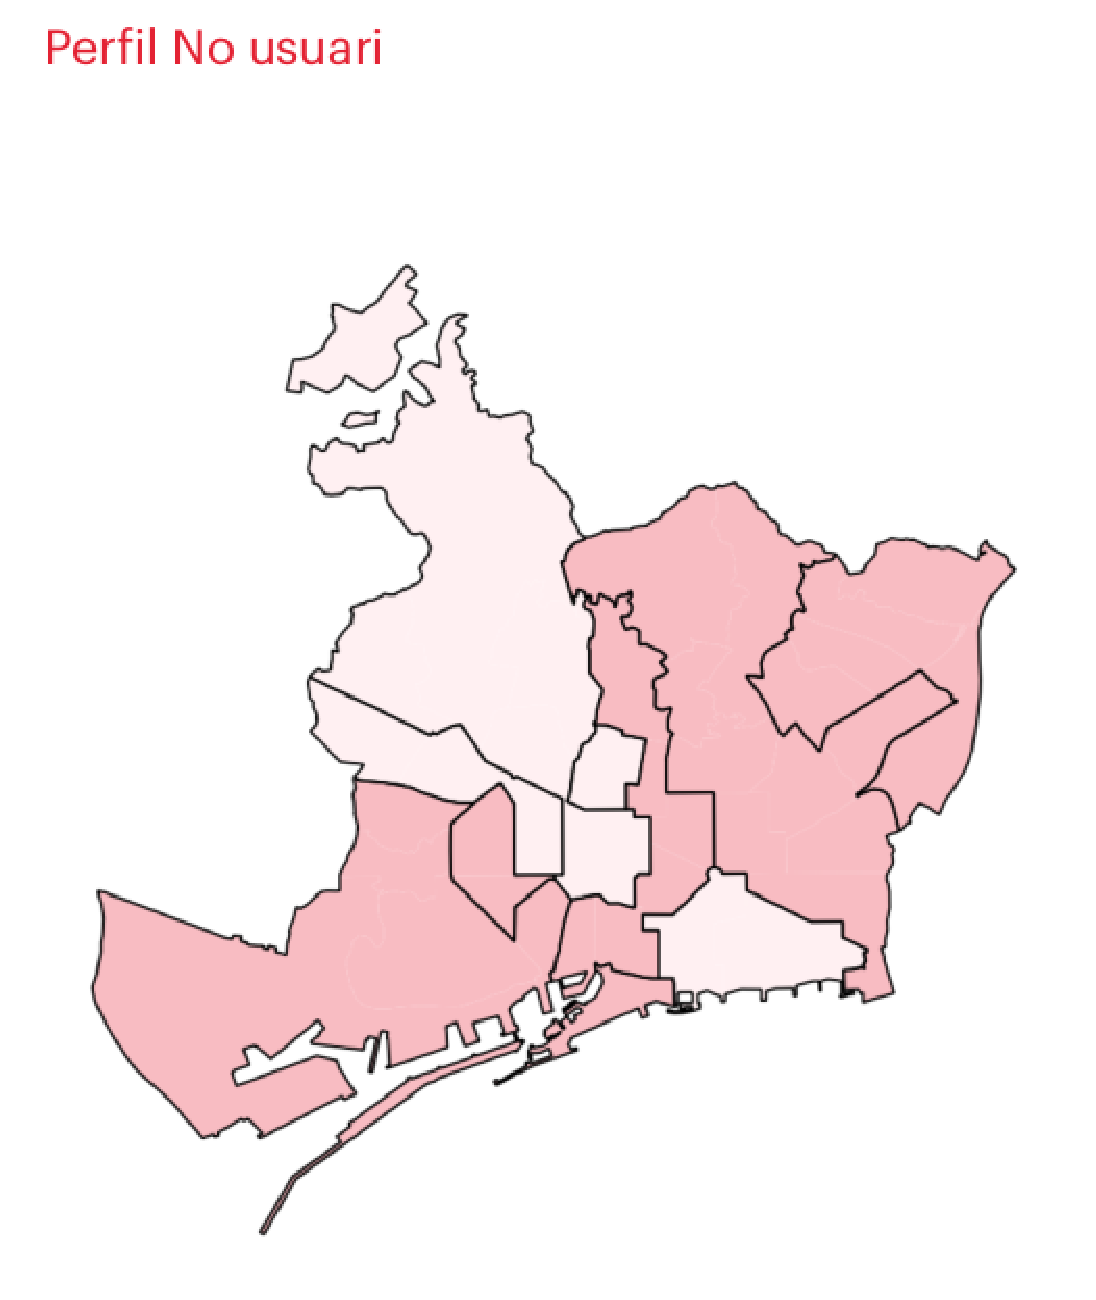
\includegraphics[width=.49\columnwidth]{fig_excletxa}
\includegraphics[width=.49\columnwidth]{fig_proposals}
%\includegraphics[width=.49\columnwidth]{fig_proposals}
%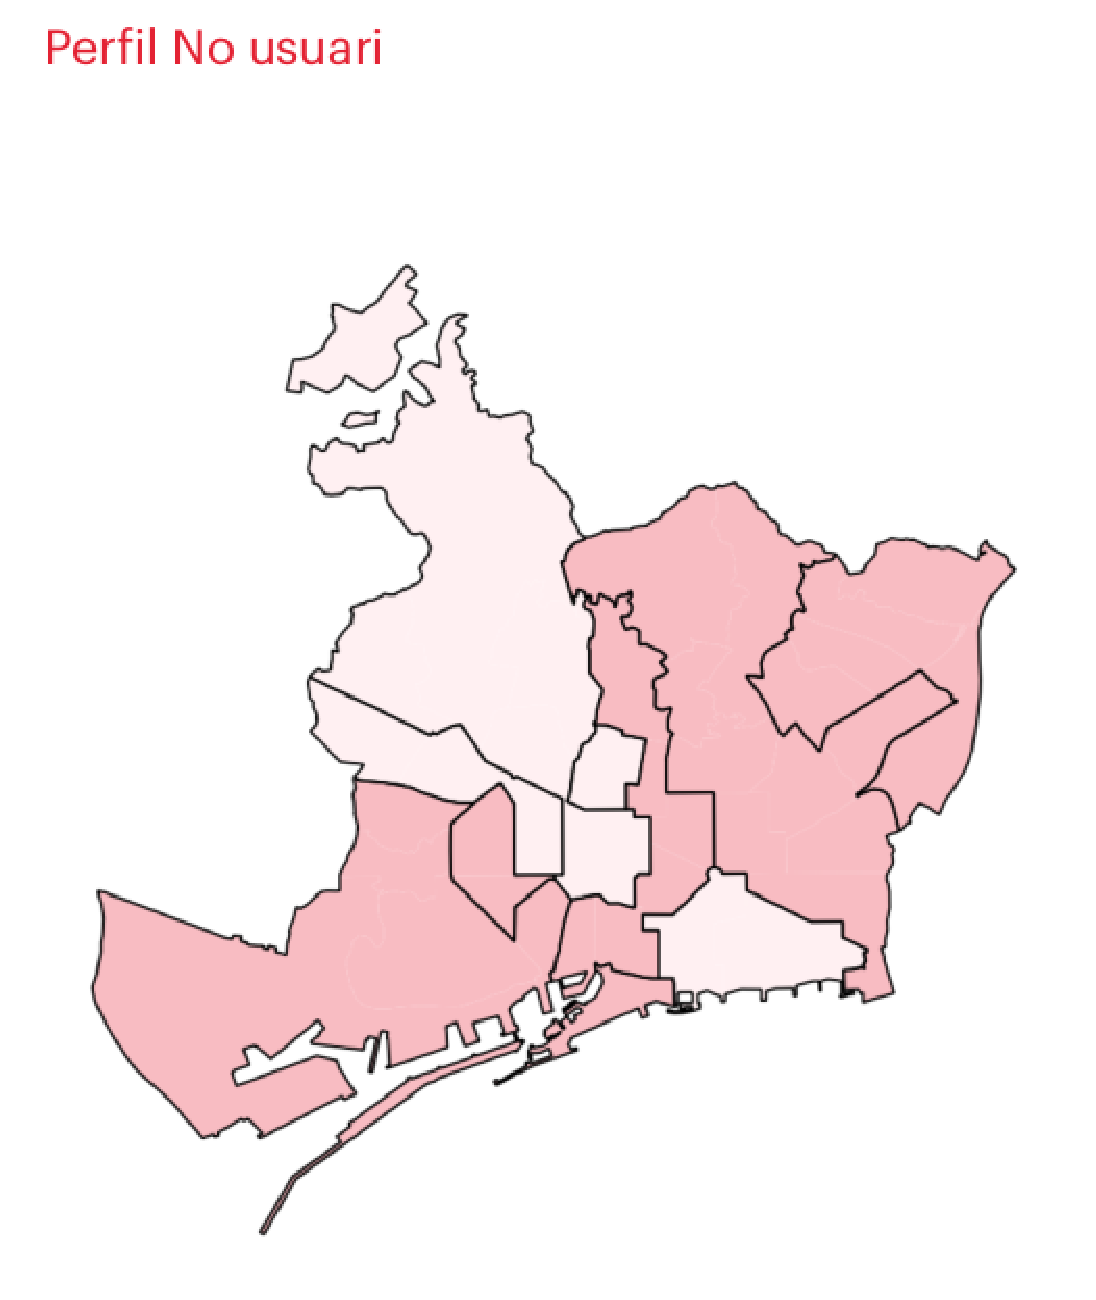
\includegraphics[width=.49\columnwidth]{fig_excletxa}
\caption{\label{fig:task1} 
L'escletxa digital i la participaci\'o per districte durant l'etapa de participaci\'o ciutadana.
A l'esquerra, el perfil digital \emph{no connectat} distribuit per nivell de renda segons~\cite{digital}.
A la dreta, un mapa on s'observa el nombre de propostas per districte.
%\footnote{hi.}.
%.
La primera part d'aquest projecte proposa caracteritzar (i corregir en la mesura del possible)
la influ\`encia de l'escletxa digital a Barcelona en la plataforma \texttt{decidim.barcelona}
utilitzant dades de diferents fonts.}
\end{figure}


En el context d'aquest projecte aquest biax selectiu est\`a principalment capturat per l'anomenada escletxa digital. 
\emph{L'escletxa digital fa refer\`encia a la desigualtat entre les persones que poden tenir acc\'es o coneixement en relaci\'o a les
noves tecnologies i les que no}~\cite{digital}.
L'informe~\cite{digital} ha posat de manifest l'exist\`encia d'aquest problema a la ciutat de Barcelona. Entre altres resultats, es posa de manifest que un de cada quatre ciutadans \'es usuari b\`asic o espor\`adic d'Internet. 
Algunes variables claus per determinar el tipus de perfil d'usuari d'Internet s\'on l'edat i el nivell d'estudis. 
\emph{Tenir una edat avan\c{c}ada, amb un baix nivell d'estudis, treballar en tasques de la llar o
ser jubilat i viure en barris de renda baixa augmenten les probabilitats de ser usuari b\`asic, espor\`adic o directament no ser usuari d'Internet}.
Des d'aquest punt de vista, el proc\'es de recol$\cdot$lecci\'o de dades online
a la plataforma \texttt{decidim.barcelona} est\`a afectat per un biaix selectiu degut a l'escletxa digital, on sectors significants de la poblaci\'o no hi s\'on representats i d'altres en s\'on sobre-representats.
La Figura~\ref{fig:task1} (esquerra) mostra un exemple del perfil no connectat distribu\"it per nivell de renda~\cite{digital}.
A l'esquerra, el perfil digital \emph{no connectat} distribuit per nivell de renda.
A la dreta, un mapa on s'observa el nombre de propostas per districte
\footnote{\texttt{https://matteodecidimbcn.carto.com/viz/3f484bd0-4cd7-11e6-9a4f-0ee66e2c9693/public\_map}}.

\textbf{El primer objectiu d'aquest projecte \'es corregir i contrastar el biaix selectiu produ\"it en el proc\'es de participaci\'o a \texttt{decidim.barcelona}}.

Com s'ha comentat anteriorment, \'es important destacar l'exist\`encia d'un proc\'es participatiu \emph{offline}, caracteritzat per l'esfor\c{c} de fer arribar les reunions presencials a tots els diferents \`ambits territorials de la ciutat.
A la dreta de la Figura~\ref{fig:task1} s'observa la representaci\'o participativa dels diferent districtes en forma d'activitats presencials.
Aquest proc\'es, si b\'e no resta exempt de possible biaix selectiu, no est\`a tant afectat per l'escletxa digital i suposa efectivament una eina per corregir i contrastar el biaix produ\"it en 
el proc\'es \emph{online}, que \'es un dels objectius d'aquest projecte.

Existeixen diferents t\`ecniques i metodologies per tractar de corregir el biaix selectiu~\cite{huang2006correcting,cortes2008sample,cortes2015adaptation}.
La t\`ecnica m\'es utilitzada consisteix en realitzar una reponderaci\'o de les dades observades.
Aquestes correccions es realitzen a partir d'una estimaci\'o m\'es objectiva que no estigui influenciada per mateix biaix.
En el marc d'aquest projecte, \'es realista pensar que aquest m\`etode \'es aplicable, ja que existeixen moltes dades poblacionals digitalitzades, com per exemple, les dades del cens electoral o del padr\'o municial. A m\'es a m\'es, es compta amb l'avantatge del proc\'es de reunions presencials que ha evolucionat en paral$\cdot$lel al proc\'es \emph{online}, suposant una font de dades molt valuable per  realitzar aquest tipus correccions.
 
La metodologia principal, doncs, consistir\`a en el creuament de diferents bases de dades per tal de calcular la corresponent reponderaci\'o estad\'istica i poder aplicar correccions a les estimacions de participaci\'o ciutadana actuals.

Les accions a desenvolupar en aquest an\`alisi seran les se\"uents:
\begin{description}
\item[1.1:-] Caracteritzaci\'o quantitativa de l'impacte de l'escletxa digital en la plataforma digital \texttt{decidim.barcelona}.
Aquesta acci\'o requereix el creuament de dades provinents de la plataforma \texttt{decidim.barcelona} (processos online i presencials) com altres possibles dades no esbiaixades (cens electoral o padr\'o municipal, per exemple), aix\'i com les dades de l'informe~\cite{digital}.
\item[1.2:-] Correccions de les mesures actuals de participaci\'o ciutadana que no contemplen aquest tipus de biaix selectiu.
Aquesta acci\'o donar\`a lloc a una reponderaci\'o de les mesures de participaci\'o juntament amb una estimaci\'o del la incertesa estad\'istica (en forma d'intervals de confianc\c{c}a) per aquelles participacions infra-representades.
\item[1.3:-] Identificaci\'o possibles usos futurs d'aquestes t\`ecniques implementades.
Per exemple, servir de suport a la presa de decisions per tal de fomentar l'\'us de tecnologies digitals en contextes particulars,
o el disseny de mecanismes a implementar en la mateixa plataforma per tal d'associar un indicador quantitatiu de (sobre)-representaci\'o de determinats usuaris o col$\cdot$lectius en detriment d'altres.

\end{description}

\subsection{Decisions sobre les propostes i creaci\'o d'actuacions}
\label{partII}
La segona part d'aquest projecte considera el proc\'es de decisi\'o mitjan\c{c}ant el qual les propostes s'han acceptat o rebutjat. Aquest proc\'es ha estat portat a terme per l'equip de govern i ha consistit en la revisi\'o, agrupaci\'o i reelaboraci\'o de les propostes provinents de la ciutadania (organitzada i no organitzada) juntament amb les cites presencials i de l'Ajuntament.
%Les actuacions s'han definit tenint en compte en qu\`e estan basades les propostes, el n\'umero de suports que han rebut, els comentaris realitzats a cadascuna, i les cites presencials associades amb elles.


\begin{figure}[t!]
\centering
\includegraphics[width=\columnwidth]{fig_proces}
\caption{\label{fig:task2} 
Associaci\'o entre propostes i decisions.
La segona part del projecte consisteix en construir un model matem\`atic (en vermell, part central) a partir de les dades 
visibles a la plataforma \texttt{decidim.barcelona} (descriptors de les propostes, en blau a la dreta) 
per poder extreure autom\`aticament el coneixement interpretable del proc\'es de que ha donat lloc a les decisions d'acceptaci\'o o rebuig de les propostes
(part dreta de la figura).
}
\end{figure}

\textbf{El segon objectiu d'aquest projecte \'es extreure el coneixement autom\`aticament de les dades 
de la plataforma \texttt{decidim.barcelona} per tal d'entendre millor el mecanisme de decisions sobre l'acceptaci\'o/rebuig de les propostes}.
L'enfoc es basa en modelar expl\'icitament el proc\'es que ha assignat a cada proposta una decisi\'o utilitzant m\`etodes anal\'itics basats en dades~\cite{Murphy}.
Concretament, es formalitzar\`a el problema d'extracci\'o de coneixement com un problema d'aprenentatge autom\`atic semi-supervisat amb estructura.
En aquesta formulaci\'o, cada proposta t\'e associades un conjunt de caracter\'istiques descriptives o predictors. Per exemple, el n\'umero de vots, l'eix en el qual est\`a definida,
el contingut (text) de la proposta, la localitzaci\'o (districte), etc. En general, qualsevol dada associada a una proposta que hagi estat mesurada.
Aquestes variables es poden representant mitjan\c{c}ant una matriu $n\times p$ de dades, on $n$ \'es el n\'umero de propostes ($10,859$) i $p$ \'es el n\'umero de descriptors
(encara per determinar). La Figura~\ref{fig:task2} (blau, esquerra) pret\'en il$\cdot$lustrar aquesta representaci\'o.

D'altra banda existeixen les variables resposta. En el nostre cas definides com la decisi\'o d'acceptar o rebutjar una proposta, juntament amb quines actuacions s'han relacionat i el text argumental en cas que la proposta fou rebutjada.
Aquesta estructura particular en les variables resposta (classificaci\'o bin\`aria juntament amb una estructura complexa d'interaccions amb les actuacions aix\'i com l'exist\`encia de llenguatge natural) representa una oportunitat i un problema interessant que no es pot adre\c{c}ar mitjan\c{c}ant m\`etodes tradicionals d'aprenentatge autom\`atic.
Aquestes apareixen a la Figura~\ref{fig:task2} a la dreta, com a \emph{decisions}, en verd o vermell.

La formalitzaci\'o d'aquest problema en termes matem\`atics inclou un model predictiu que \'es capa\c{c} de transformar els predictors en variables resposta.
\'Es aquest model predictiu l'objecte a desenvolupar en aquesta part del projecte.
El model cont\'e uns par\`ametres (o graus de llibertat) els valors dels quals s'estableixen resolent un problema d'optimitzaci\'o matem\`atica. T\'ipicament es minimitza l'error entre les variables resposta i les prediccions del model a partir de les variables predictores.

\'Es important que el model predictiu sigui interpretable, \'es a dir, sigui avinent per fer extracci\'o de coneixement.
\'Es bastant freq\"uent en aquest tipus d'an\`alisi utilitzar models de caixa negra (\emph{black box models}), on la interpretabilitat del model queda sacrificada per tal d'obtenir m\'es poder predictiu. 
En aquest projecte aquesta limitaci\'o s'adre\c{c}ar\`a fent servir models senzills, on la soluci\'o del problema sigui \'unica i interpretable. Hi ha v\`aries t\`ecniques per aconseguir-ho, totes passen per for\c{c}ar estructura en la soluci\'o del problema que, de manera agn\`ostica, resulti en un problema amb una \'unica soluci\'o \`optima global.

Una possible limitaci\'o important per assolir aquest segon objectiu \'es la pres\`encia d'un altre tipus de biaix, diferent al biaix de selecci\'o mencionat en l'apartat anterior. En aquest cas, produ\"it per l'exist\`encia de variables latents, les quals no han estat mesurades. Aquestes variables, doncs, no formen part del conjunt de predictors, per\`o poden tenir una influ\`encia significativa en el proc\'es per determinar si una proposta ha estat acceptada o no. Per exemple, en el cas que ens ocupa, variables latents poden representar criteris de decisi\'o que puguin haver estat contemplats durant la revisi\'o, agrupaci\'o i reelaboraci\'o de les propostes i que no apareguin expl\'icits en cap lloc de la plataforma.

L'exist\`encia d'aquestes variables \emph{frustrades} (en angl\`es \emph{confounders}) provoca que el model no sigui indentificable, que vol dir que no es puguin tra\c{c}ar relacions de causalitat entre les variables predictores i les variables resposta~\cite{Pearl}. No obstant, 
aix\`o no impedeix poder caracteritzar i establir correlacions i depend\`encies estad\'istiques robustes que 
serveixin per identificar les variables m\'es rellevants alhora de predir si una proposta ha estat acceptada o no.

La metodologia principal, doncs, d'aquesta part consistir\`a en l'aprentatge autom\`atic d'un model anal\'itic a partir de les dades associades a cada proposta i resultats del pla d'actuaci\'o que permeti caracteritzar el proc\'es de decisi\'o a la plataforma.

Les accions a desenvolupar en aquesta segona part seran les seg\"uents:
\begin{description}
\item[2.1:-] 
An\`alisi quantitatiu de la interacci\'o de les diferents caracter\'istiques descriptives de les propostes i la 
relaci\'o d'interaccions entre les diferents propostes acceptades i actuacions definides.
Aquesta part \'es important per assegurar que les dades d'entrada s\'on adequades al model utilitzat.
\item[2.2:-]
Definici\'o i optimitzaci\'o d'un model matem\`atic que capturi el proc\'es de decisi\'o i que sigui interpretable.
Aquest model identificar\`a les caracter\'istiques de les propostes que estad\'isticament siguin rellevants per poder concloure el resultat d'acceptaci\'o o rebuig d'aquesta.
\item[2.3:-]
Identificaci\'o de possibles usos futurs d'aquestes t\`ecniques implementades.
Per exemple, la construcci\'o d'un sistema de recomanaci\'o autom\`atic on, d'acord a diferents criteris, 
que suporti la presa de decisions de l'equip de l'Ajuntament.
\end{description}

%
%Com s'ha comentat anteriorment, l'an\`alisi preliminar mostra una .
%Aquest es pot consultar en l\'inia a la web de .
%
% Aquestes caracter\'istiques 
%el conjunt de propostes formen una matriu  dades formen caracter\'istiques de les pro
%Aquest objectiu requereix .
%
\section{P\'ublic objectiu de la recerca i beneficis potencials generats dels resultats}

Aquest projecte clarament reconeix les pr\`actiques de participaci\'o que s\'on iniciativa de la ciutadania i aprofundeix en els mecanismes de democr\`acia i de
participaci\'o de l'Ajuntament de Barcelona.
Els resultats no nom\'es s\'on inter\`es cient\'ific tant en l'\`ambit socio-pol\'itic com el computacional i estad\'istic, sino que, a m\'es a m\'es, generaran una utilitat directa en forma d'eines implementades directament a la plataforma. Per tant, 
aquest projecte tamb\'e ajuda a avan\c{c}ar en la coproducci\'o de pol\'itiques públiques.

La tasca de quantificar la influ\`encia de l'escletxa digital en \texttt{decidim.barcelona}, l'eina m\'es important de democr\`acia participativa del govern, \'es imprescindible per garantir un grau de participaci\'o de persones i col$\cdot$lectius en risc de ser invisibilitzats en el disseny i execuci\'o de les pol\'itiques participatives actuals, tenint en compte diversitat d'origen, diversitat funcional, paritat per sexe i altres.
%projecte tenint en compte
%
El projecte tamb\'e aprofundeix en la col$\cdot$laboraci\'o entre Ajuntament i el teixit associatiu pel que fa a la gesti\'o d'all\`o p\'ublic.

El model desenvolupat a la segona part del projecte \'es rellevant per diferents raons.
Primera, generar models matem\`atics que permetin explicar de manera objectiva quins valors influeixen en les valoracions de l'equip de govern facilita la transpar\`encia.
Segona, adre\c{c}a un dels reptes actuals m\'es importants de donar sentit als grans volums de dades que la nostra societat genera.
Important, el model proposat \'es interpretable, validable i tamb\'e modificable. Des d'aquest punt de vista, la presa de decisions i l'automatizaci\'o van lligades i depenen del factor hum\`a, evitant possibles efectes de discrimiaci\'o algor\'itmica.

\section{Pla de treball}
El projecte ser\`a coordinat pel sol$\cdot$licitant que realitzar\`a les tasques de supervisi\'o i seguiment continuat. Donat que el grau d'interdepend\`encia entre les dues parts del projecte es baix, aquest es pot entendre com dos sub-projectes relativament independents. Es proposaran dos projectes associats a un programa de m\`aster o d'inici de doctorat.
Per tant, existir\`a un proc\'es de selecci\'o de diferents candidats o candidates que siguin competents i mostrin un grau alt de motivaci\'o. La selecci\'o de candidats o candidates incorporar\`a la perspectiva de g\`enere.

L'equip de treball format pel coordinador i els candidats(es) seleccionats(es) establir\`a una col$\cdot$laboraci\'o continuada amb les entitats relacionades. Principalment, amb l'equip de govern encarregat de desenvolupar
la plataforma online, incloent el grup Tecnopol\'itica IN3/UOC, Internet Interdisciplinary Institute (IN3) i l'associaci\'o aLabs, aix\'i com
altres entitats relacionades. Aquesta col$\cdot$laboraci\'o comportar\`a l'assist\`encia a reunions peri\`odiques i l'elaboraci\'o d'informes on es faci expl\'icit el progr\'es del projecte.
En tot moment, es garantir\`a la privacitat i seguretat de les dades tractades.

La Taula \ref{crono} mostra una estimaci\'o de la cronologia del projecte en el cas que les dues tasques
principals es desenvolupin en paral$\cdot$lel per dues persones, juntament amb el coordinador.
\begin{table}[!h]
\centering
\caption{Cronologia aproximada del projecte}
\label{crono}
\begin{tabular}{|l|l|l|l|l|l|l|l|}
\hline
\multicolumn{1}{|c|}{\textbf{Part del projecte}}       & \multicolumn{7}{c|}{\textbf{Accions relacionades}}                                                                                                                                                        \\ \hline
Part I (secci\'o \ref{partI})    & \multicolumn{2}{c|}{\cellcolor[HTML]{34CDF9}1.1} & \multicolumn{3}{|c|}{\cellcolor[HTML]{96FFFB}1.2} & \multicolumn{2}{c|}{\cellcolor[HTML]{67FD9A}1.3}\\ \hline
Part II (secci\'o \ref{partII}) & \multicolumn{2}{c|}{\cellcolor[HTML]{34CDF9}2.1}   & \multicolumn{4}{|c|}{\cellcolor[HTML]{96FFFB}2.2}               & \cellcolor[HTML]{9AFF99}2.3\\ \hline
\multicolumn{1}{|r|}{Temps (mesos)}                    &      1                            &2                                 &3                      &4                     &5                     &6             &7 $\rightarrow$                                                    \\ \hline
\end{tabular}
\end{table}

En cas que nom\'es un candidat o candidata sigui escollit, les tasques es redistribuiran seq\"uencialment i l'experi\`encia
adquirida durant la primera tasca permetr\`a reduir el temps de desenvolupament de la segona.
El cap cas el temps total de desenvolupament mai sobrepassar\`a els $12$ mesos.
Al final de cada acci\'o, es lliurar\`a un informe per fer expl\'icit el seguiment i l'avaluaci\'o continuada del projecte.
Al final de cada part, s'elaborar\`a un entregable que inclogui tots els resultats corresponents a la part desenvolupada.

Es preveu la publicaci\'o dels resultats cient\'ifics en confer\`encies i/o revistes cient\'ifiques relacionades. Exemples de confer\`encies poden ser \emph{The Internet, Policy \& Politics Conference}, \emph{Knowledge Discovery and Data Mining} o \emph{European Conference on Machine Learning and Principles and Practice of Knowledge Discovery}.

\section{Pressupost}
El pressupost del projecte inclou principalment dues ajudes a estudiants que estiguin finalitzant els seus estudis de m\`aster o comen\c{c}ant el doctorat, aix\'i com despeses d'equipament inform\`atic i altres despeses associades a la publicaci\'o d'articles, com registres a confer\`encies internacionals i viatges.
La Taula~\ref{press} resumeix els costs.
\begin{table}[!h]
\centering
\caption{Pressupost}
\label{press}
\begin{tabular}{lr}
\hline
\multicolumn{1}{|l|}{\textbf{Concepte}}                                            & \multicolumn{1}{l|}{\textbf{Cost}}        \\ \hline
\multicolumn{1}{|l|}{Estudiant nivell master / inici PhD}                 & \multicolumn{1}{r|}{5,500 \euro} \\ \hline
\multicolumn{1}{|l|}{Estudiant nivell master / inici PhD}                 & \multicolumn{1}{r|}{5,500 \euro} \\ \hline
\multicolumn{1}{|l|}{Equipaments: dos laptops}                            & \multicolumn{1}{r|}{3,000 \euro} \\ \hline
\multicolumn{1}{|l|}{Despeses en registres confer\`encies internacionals} & \multicolumn{1}{r|}{4,000 \euro} \\ \hline
\multicolumn{1}{r}{Total}                                                 & \multicolumn{1}{l}{18,000 \euro}
\end{tabular}
\end{table}

%\section{Documentaci\'o addicional}

\section{Capacitats per l'elaboraci\'o del projecte}
El sol$\cdot$licitant del projecte t\'e \`amplia experi\`encia en el tractament de grans volums de dades i una traject\`oria cient\'ifica internacional rellevant en l'\`area d'aprentatge autom\`atic i de m\`etodes estad\'istics i computacionals.
El projecte \'es desenvolupar\`a principalment en un entorn de treball universitari, on es disposen dels recursos necessaris
per poder definir l'equip de treball de manera \`optima i desenvolupar el projecte satisfact\`oriament.

Per raons d'anonimitat, aquesta secci\'o est\`a m\'es elaborada en el document addicional, on figuren les dades de l'aplicant.

%\section{Antecedents i estat actual del tema}
%\emph{Tamb\'e a nivell internacional (m\`axim 2 p\`agines)}
%
%
%\section{Objectius i justificaci\'o de l'estudi}
%\emph{Especifiqueu breument els objectius que cal assolir i l'adequaci\'o a les bases, fent especial menci\'o a l'inter\`es i novetat que representa el projecte i justificaci\'o del seu encaix en els \`ambits tem\`atics inclosos en la convocat\`oria (m\`axim 2 p\`agines)}
%
%this is a citation~\cite{dcent}
\newpage
\bibliographystyle{plain}
\bibliography{references}

\end{document}
% End of v2-acmsmall-sample.tex (March 2012) - Gerry Murray, ACM


